\newpage
\section{Golden Ratio} %% remove * if added to main notes


\begin{question} Is the golden ratio constructible?\index{golden!ratio} 
\end{question}
\QM

Well 
\[
\phi =\frac{1 + \sqrt{5}}{2},
\]
so of course it is. But, how do you actually construct it? Here is an easy way:

\begin{construction}[Golden Ratio]\index{compass and straightedge!golden ratio}\index{golden!ratio!compass and straightedge} \hfill
\begin{enumerate}
\item Consider a unit on a line.
\item Construct a perpendicular of unit length at the right end point of the unit.
\item Bisect the original unit.
\item Draw an arc, centered at the point found in Step $3$ that goes 
through the top of the perpendicular drawn in Step $2$.
\item The segment starting at the left end of the unit and ending at the point found in Step $4$ is of length $\phi$.
\end{enumerate}
\[

\includegraphics{../graphics/phi.pdf}
\]
\end{construction}


\begin{question}\index{compass and straightedge!pentagon}\index{pentagon}How how do you construct a regular pentagon? 
\end{question}
One way is to use golden triangles:\index{golden!triangle}
\[
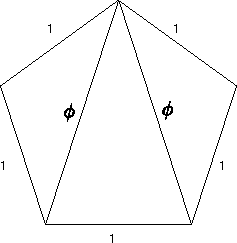
\includegraphics{../graphics/pentagon.pdf}
\]

What about other regular $n$-gons?  \index{Gauss, Carl Friedrich}Carl
Friedrich Gauss, one of the greatest mathematicians of all time,
solved this problem when he was 18. He did this around the year 1800,
nearly 2000 years after the time of the Greeks.  How did he do it?  He
thought of constructions algebraically as we have been doing. Using
these methods, he discovered this theorem:


\begin{theorem}[Gauss]\label{T:gauss}  One can construct a regular $n$-gon if $n\ge 3$ and 
\[
n= 2^i \cdot p_1\cdot p_2\cdots p_j
\]
where each subscripted $p$ is a distinct prime number of the form
\[
2^{(2^k)}+1
\]
where  $i$, $j$, and $k$ are nonnegative integers.
\end{theorem}\index{prime numbers}

Around thirty years later, Wantzel\index{Wantzel, Pierre} proved that
these were the only regular polygons that could be constructed.

\begin{question} Find $i$, $j$, and $k$ for a regular $3$-gon, $4$-gon, $5$-gon, and $6$-gon.
\end{question}
\QM
